\documentclass[11pt]{article}

\usepackage[margin=1in]{geometry}
\usepackage{setspace}
\usepackage{titlesec}
\usepackage{booktabs}
\usepackage{float}
\usepackage{tabularx}
\usepackage{graphicx}

\titleformat{\section}{\large\bfseries}{\thesection}{1em}{}
\titleformat{\subsection}{\normalsize\bfseries}{\thesubsection}{1em}{}

\title{\textbf{Deliverable 2 — Preliminary Results}\\
Introduction to Machine Learning}
\author{
Gonçalo Almeida (119792) \\
Margarida Ribeiro (119876) \\
João Barreira (120054)
}
\date{}

\begin{document}

\maketitle

\onehalfspacing

\section{Data Processing Methodology}

\paragraph{}Data preparation is a critical step in the lifecycle of any Machine Learning project, especially in complex domain scenarios such as anomaly detection in network traffic. The CIC-IDS2017 dataset presents characteristics inherent to real-world data: high volume, the presence of corrupted or missing values, as well as class imbalance.

The processing pipeline was designed with resource optimisation and statistical reliability in mind, structured across the following phases.

\subsection{Data Ingestion and Sampling}

\paragraph{}The dataset totals more than 1GB of traffic, spread across multiple CSV files corresponding to several days of capture. Given the redundancy of normal patterns, the data was aggregated and a 20\% Stratified Sampling was applied. This technique ensured that the generated sample faithfully maintains the same proportion of benign instances (80.3\%) and anomalies (19.7\%) present in the original dataset, resulting in a data volume of around 565 thousand instances, which is well-suited to the memory requirements of algorithms in an offline environment (such as Isolation Forest) during the rapid experimentation cycle.

\subsection{Data Cleaning}

\paragraph{}During the exploratory phase (Deliverable 1), formatting issues and invalid values were identified:

\begin{enumerate}

    \item \textbf{Structural Cleaning:} Residual whitespace in column names was removed, which is critical to avoid discrepancies in intermediate calls during analysis (e.g. restoring \texttt{ Flow Duration} to \texttt{Flow Duration}).
    \item \textbf{Handling Missing and Infinity Values:} Although residual (affecting approximately 2800 instances, i.e., \verb|<|0.1\% of the dataset), the presence of infinite values (due to divisions by zero during feature extraction from the pcap, e.g.: \texttt{Flow Bytes/s}) or null values (\texttt{NaN}) directly impacts mathematical models sensitive to numerical domains. Full exclusion (Drop) of these rows was chosen (\texttt{dropna}), assuming that their reduced prevalence does not translate into a loss of useful behavioural context. Imputing data for a case of "infinite packet speeds" would not reflect organic network behaviour, introducing bias.
\end{enumerate}

\subsection{Feature Engineering Selection}

\paragraph{}Adapting the dataset columns to the model requires reducing noise and unnecessary dimensionality.

\begin{itemize}
    \item \textbf{Zero Variance Check:} 8 features that demonstrated zero variance across the network captures were removed (e.g. \texttt{Bwd PSH Flags}, \texttt{Bwd URG Flags}, \texttt{Fwd Avg Bytes/Bulk}, etc.). Static attributes limit analytical usefulness, introduce computational noise, and do not contribute the variability necessary for distance-based detections.
    \item \textbf{Label Categorisation:} In the context of this unsupervised technique (even though evaluated with labels in a binary baseline), the categorical variable for traffic type was mapped to an integer numerical domain (\texttt{0} for \texttt{BENIGN}, \texttt{1} for anomalous context). All subsequent analyses will ignore this feature in unsupervised measurements, acting only as an evaluation pillar.
\end{itemize}

\subsection{Feature Scaling and Train/Test Split}

\paragraph{}The final phase focused on the preventive preservation of informational bias (Data Leakage):

\begin{itemize}
    \item \textbf{Dataset Split:} The stratified sample was divided with a proportion of 70\% for Training (Train), 15\% for Validation, and 15\% for Testing. This single-generation split approach was chosen over Cross-Validation because the large volume of data (approx. 565,000 instances) ensures statistical significance without the prohibitive computational cost of k-fold validation. The distribution across splits is shown in Figure \ref{fig:data_dist}. This ensures sufficiently unseen instances in an independent hyper-testing environment to validate the model's true generalization capacity.
    
    \begin{figure}[H]
        \centering
        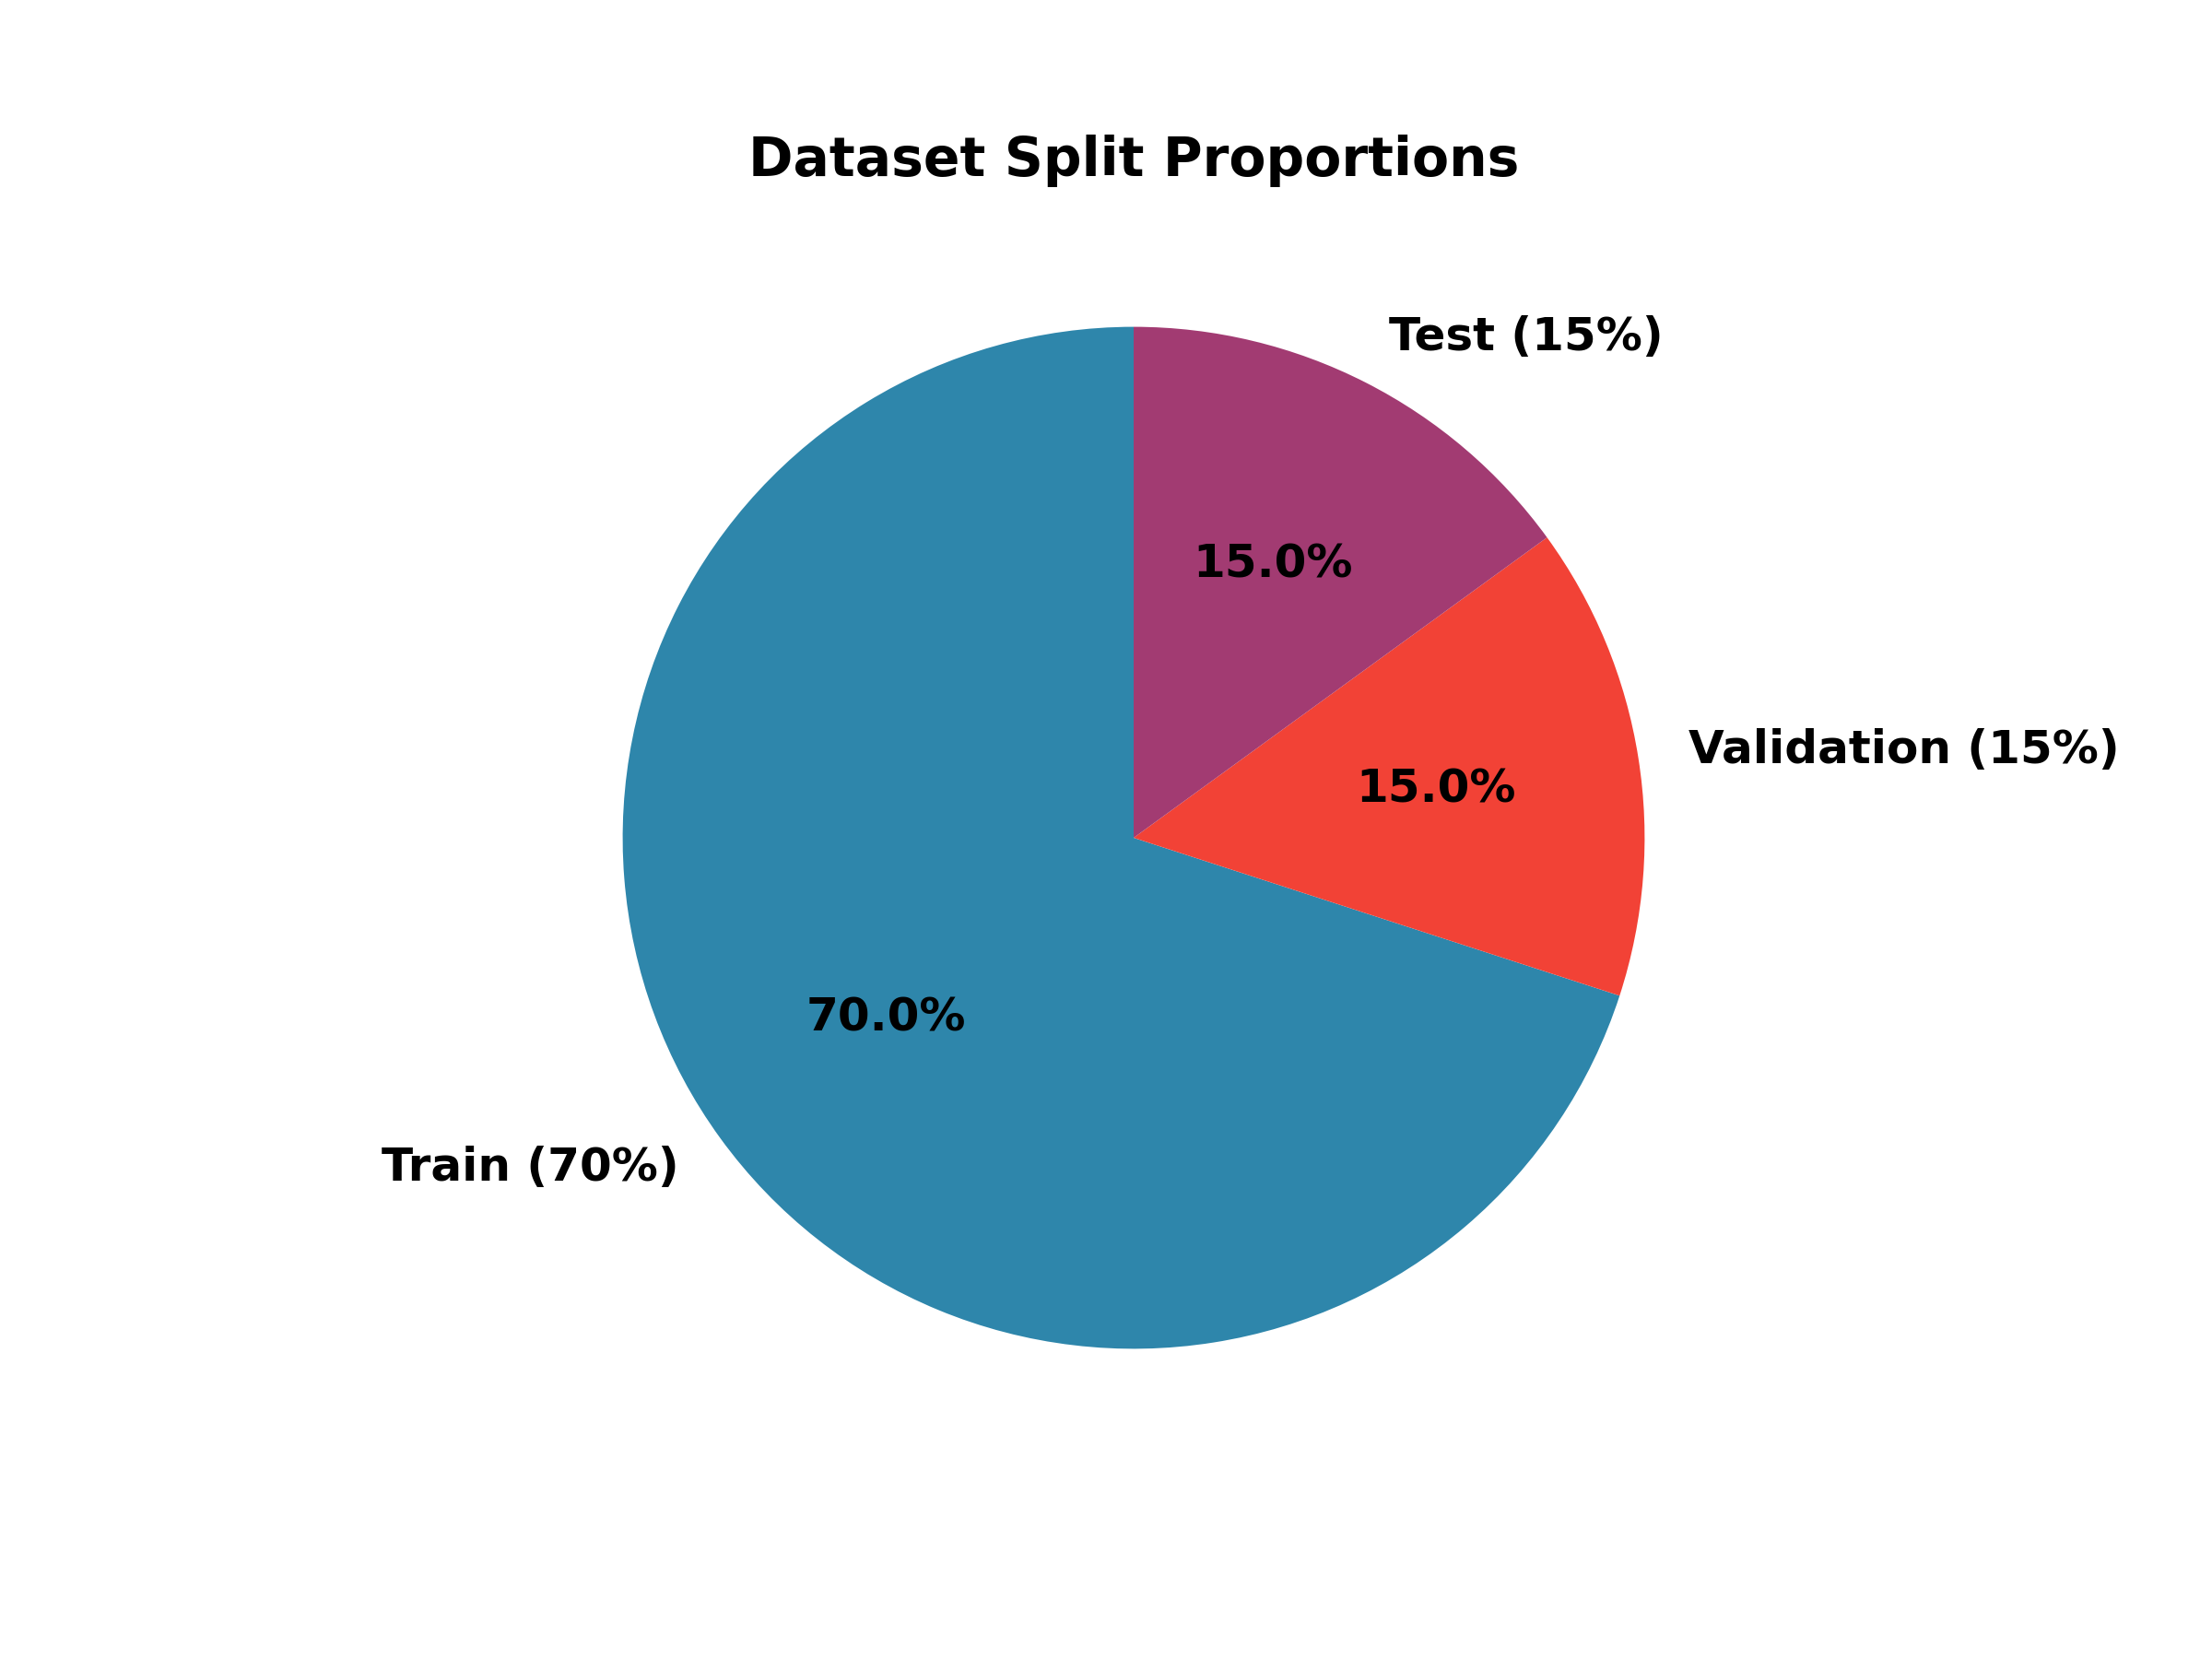
\includegraphics[width=0.48\textwidth]{../evaluation_results/dataset_split.png}
        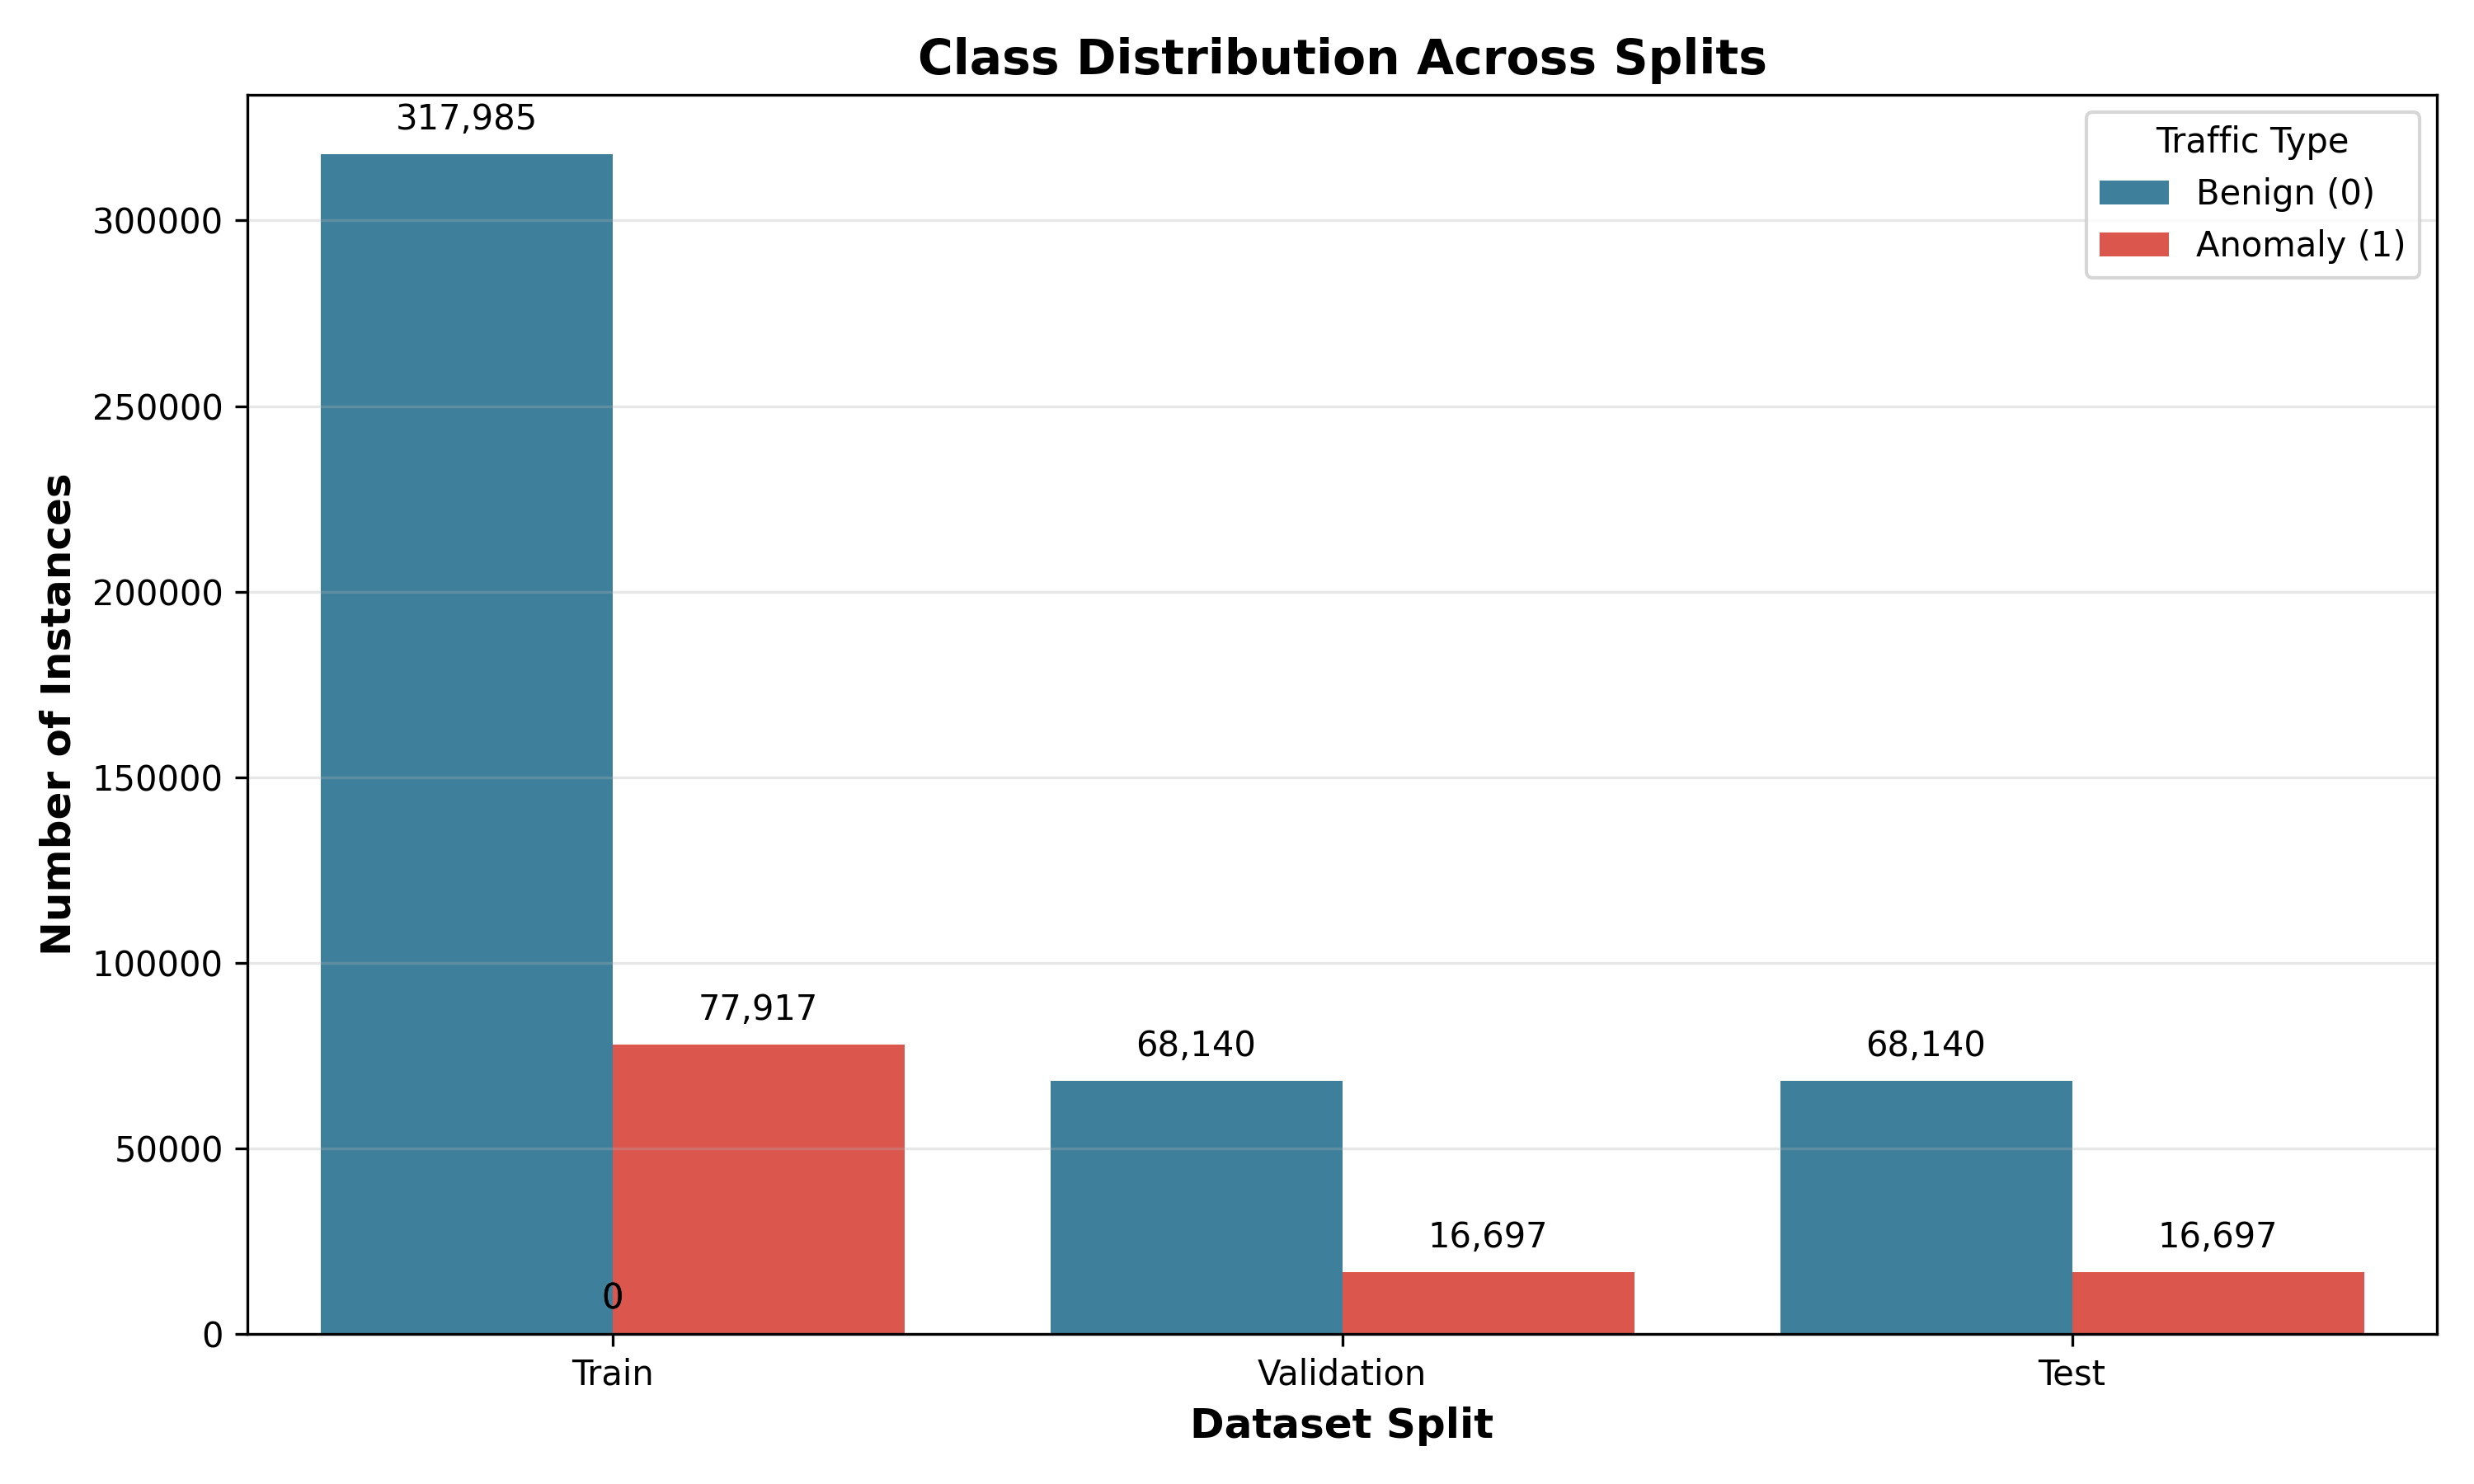
\includegraphics[width=0.48\textwidth]{../evaluation_results/class_distribution.png}
        \caption{Dataset split proportions and class distribution across train, validation, and test subsets.}
        \label{fig:data_dist}
    \end{figure}

    \item \textbf{Normalisation (Standardisation):} It was observed that metrics such as packet volume vs. flow duration vary across different orders of magnitude. Therefore, attribute normalisation was performed based on the assumption of their variation, using \texttt{StandardScaler}. Special attention was paid to the temporal scaling framework: the scaler was fit exclusively on the Train subset, subsequently transforming the validation and test sets using the same basis.
\end{itemize}

\section{Models Explored and Justification for Their Selection}

In this phase, six distinct anomaly detection algorithms were implemented and evaluated against the CIC-IDS2017 dataset, using a multi-perspective evaluation strategy to ensure robust and unbiased comparison.

\subsection{Evaluation Framework}

To address the question of generalization, it is crucial to clarify that \textbf{all results presented in this section refer exclusively to the Test set}. This unseen subset of 84,837 instances was completely isolated during training and hyperparameter tuning, ensuring that the evaluated models are effectively generalizing and not merely memorizing the training distribution.

Given the severe class imbalance inherent in the dataset (approximately 80\% normal, 20\% anomalous traffic), relying on a single metric such as accuracy would be misleading since a trivial classifier that always predicts ``normal'' would achieve 80\% accuracy while being completely useless. Three complementary evaluation perspectives were therefore adopted:

\begin{enumerate}
    \item \textbf{Original Distribution} (realistic, imbalanced): 84,837 test instances (68,140 normal, 16,697 anomalous), reflecting production conditions.
    \item \textbf{Balanced Subset} (debiased): 33,394 instances (50/50 split), to isolate true model discriminative capability from distributional bias.
    \item \textbf{Per-Class Analysis}: Separating Recall and Precision by class to understand the security-relevant trade-off between missed attacks (False Negatives) and false alarms (False Positives).
\end{enumerate}

The primary metrics used are \textbf{F1-Score}, \textbf{AUC-ROC}, \textbf{Recall} (for anomalies), and \textbf{Balanced Accuracy}. In the cybersecurity domain, \textbf{Recall (anomaly)} is the most critical metric, as a False Negative, a missed attack, is substantially more dangerous than a False Positive.

\subsection{Models and Results}

The behavior of the models when evaluated in isolation and as an ensemble on the test set is detailed below.

\begin{figure}[H]
    \centering
    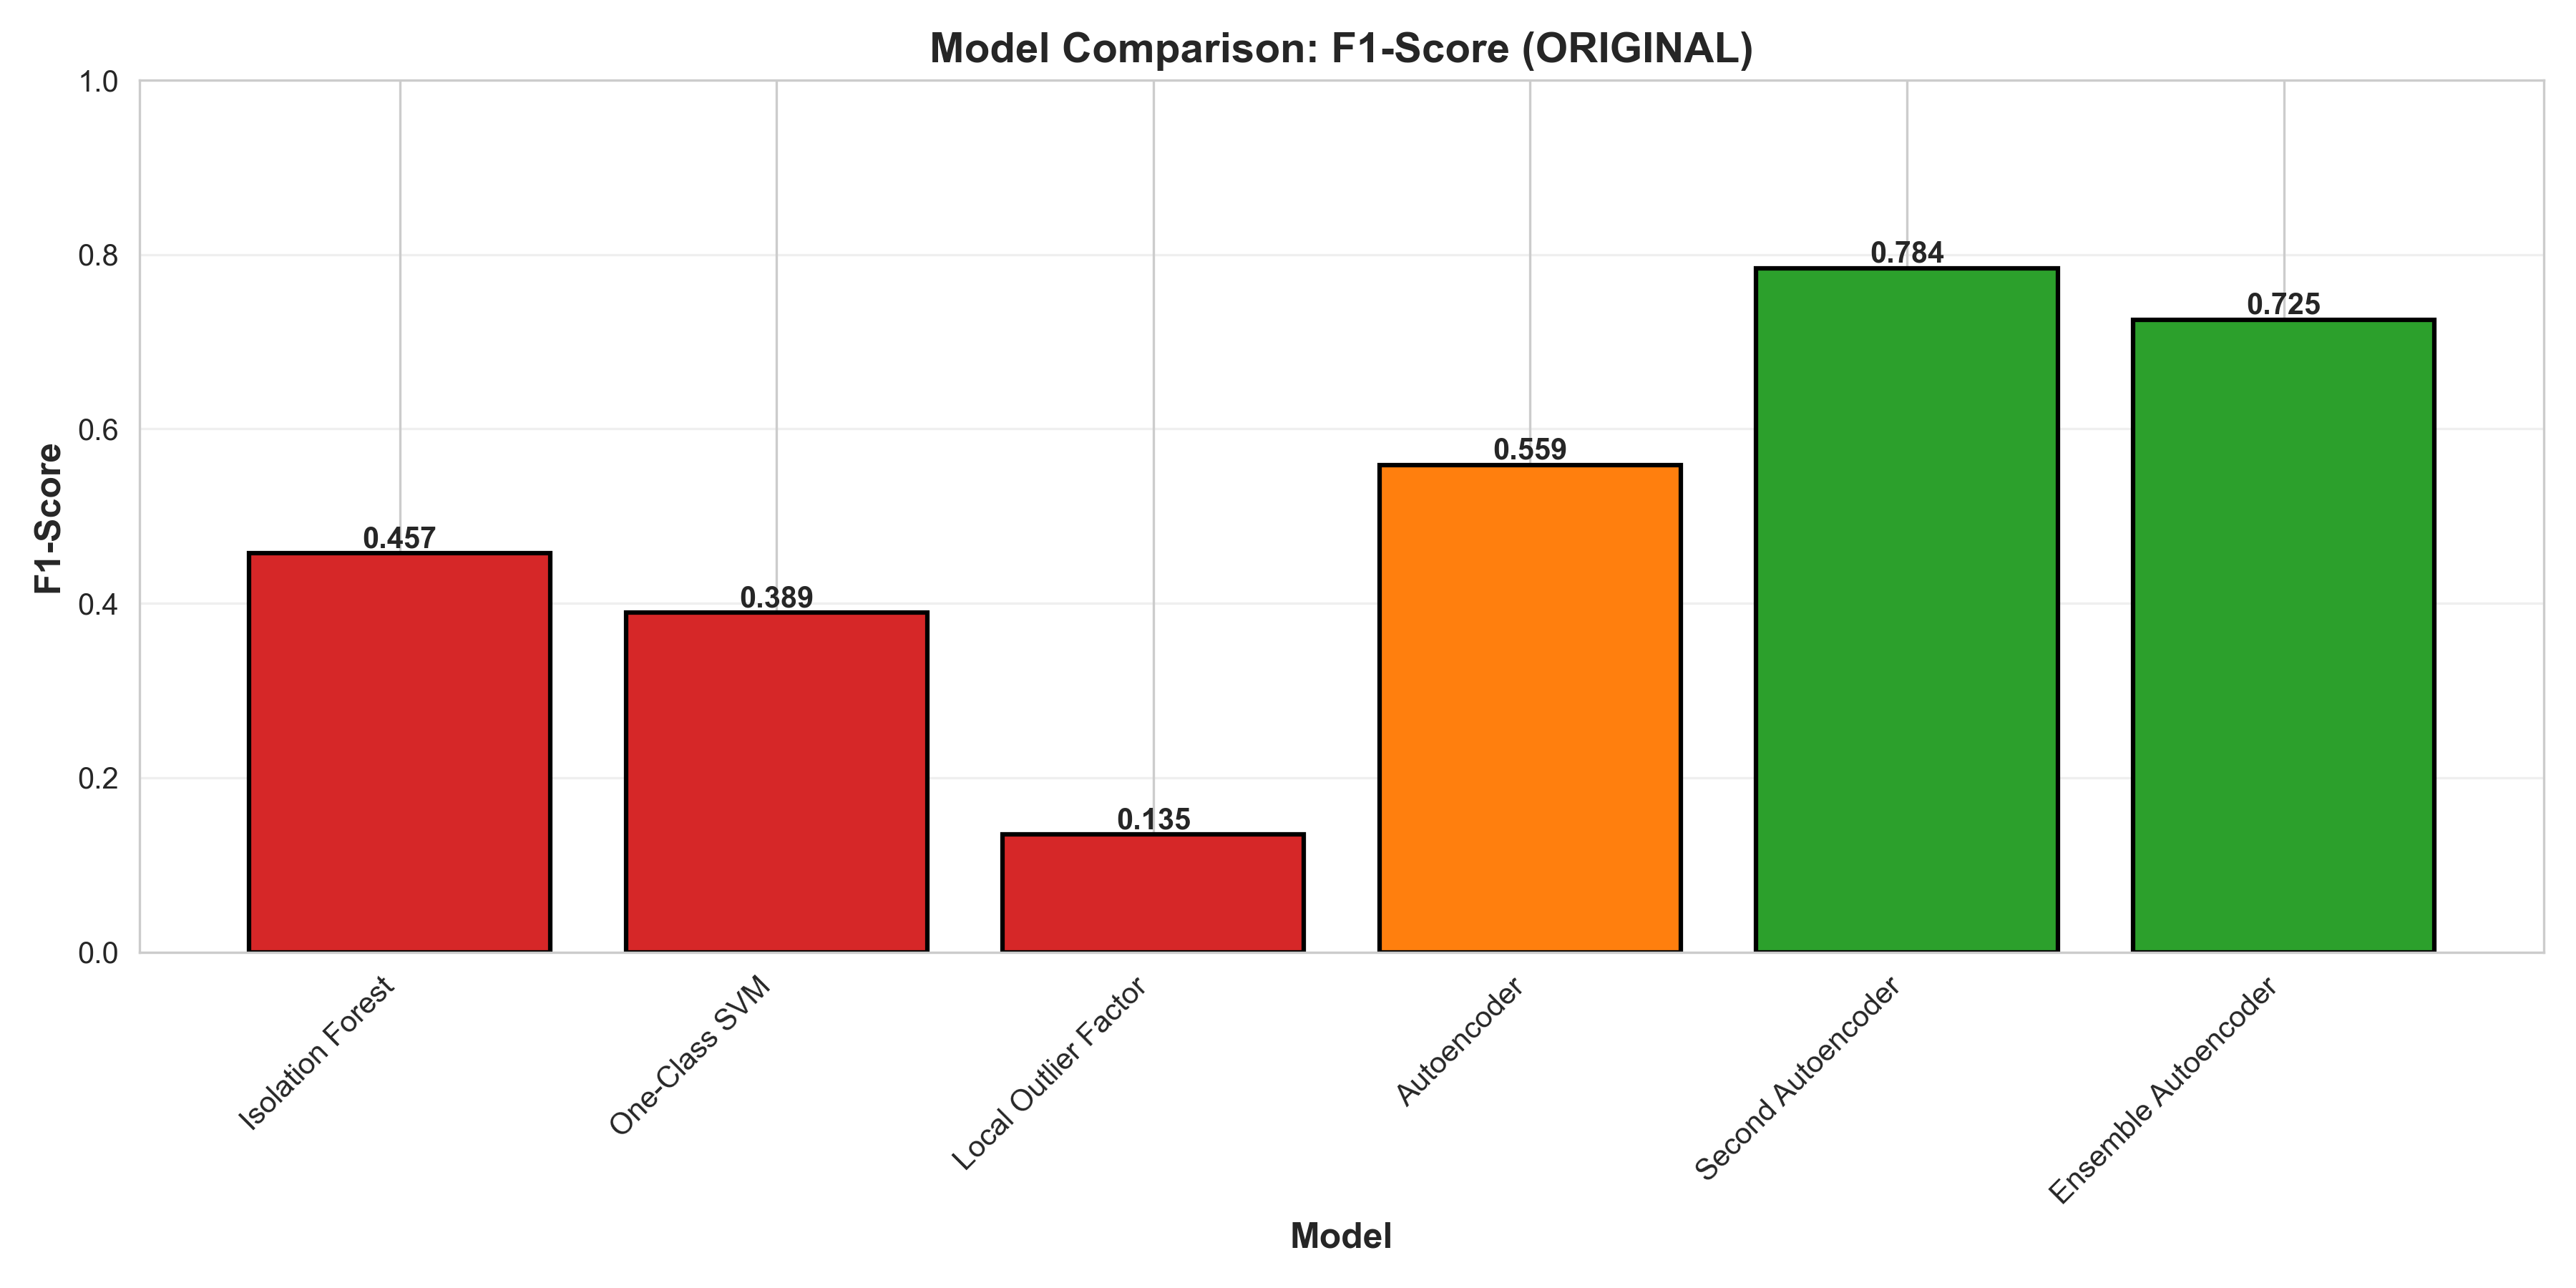
\includegraphics[width=0.8\textwidth]{../evaluation_results/comparison_f1-score_original.png}
    \caption{F1-Score comparison across evaluated models on the original imbalanced test distribution.}
    \label{fig:f1_comparison}
\end{figure}

\begin{table}[H]
    \centering
    \caption{Model Comparison — Original Distribution (Imbalanced, Realistic)}
    \begin{tabularx}{\textwidth}{lccccX}
        \toprule
        \textbf{Model} & \textbf{Precision} & \textbf{Recall} & \textbf{F1} & \textbf{AUC-ROC} & \textbf{Notes} \\ \midrule
        \textbf{Ensemble AE}         & 0.5684 & \textbf{0.9632} & 0.7149 & \textbf{0.9830} & Best security profile \\
        \textbf{Second AE}           & \textbf{0.7581} & 0.7704 & \textbf{0.7642} & 0.9451 & Best F1, fewer false alarms \\
        Primary AE                   & 0.5171 & 0.5255 & 0.5213 & 0.8482 & Good baseline \\
        Isolation Forest             & 0.4375 & 0.4500 & 0.4436 & 0.6857 & Fast; insufficient recall \\
        One-Class SVM                & 0.3804 & 0.3983 & 0.3891 & 0.6129 & Expensive; poor performance \\
        Local Outlier Factor         & 0.1308 & 0.1342 & 0.1325 & 0.4386 & Near-random; not viable \\
        \bottomrule
    \end{tabularx}
\end{table}

\subsection{Model-by-Model Justification}

\paragraph{Isolation Forest.} A tree-based ensemble that isolates anomalies by randomly partitioning the feature space. It is fast and interpretable, making it a natural baseline for anomaly detection. However, with an AUC-ROC of 0.69 and a Recall of only 45\%, it fails to detect the majority of attacks. Its precision is highly sensitive to class imbalance (44\% on original data, 76\% on balanced data), revealing that its predictions are partially driven by prior probabilities rather than genuine learned patterns. It is not recommended for production without combining it with a signature-based system.

\paragraph{One-Class SVM.} Learns a hypersphere around normal data in a kernel-projected feature space. Despite its theoretical expressiveness, it performed worse than Isolation Forest across all metrics (AUC-ROC: 0.61, Recall: 40\%). Additionally, its $\mathcal{O}(n^2)$ complexity made it very expensive, training was limited to a 10\% data subset, further undermining its suitability for large-scale network monitoring.

\paragraph{Local Outlier Factor (LOF).} Assigns anomaly scores based on local density relative to neighbours. LOF is known to struggle in high-dimensional spaces, a limitation directly observed here: with 70 features, the algorithm performed near-randomly (AUC-ROC: 0.44, Recall: 13\%). This is a well-documented consequence of the curse of dimensionality, where local density becomes meaningless as distances converge.

\paragraph{Primary Autoencoder (trained on normal traffic).} A neural network trained to reconstruct benign flows. Anomalies, which deviate from learned normal patterns, produce higher reconstruction errors and are flagged using the 80th percentile as a threshold. This model achieved a significant improvement over classical methods (AUC-ROC: 0.85), confirming that deep non-linear representations are better suited for this task. The model converged at epoch 29 (minimum loss: 0.0615). However, its Recall of 53\% was considered insufficient in isolation.

\paragraph{Second Autoencoder (trained on anomalous traffic).} An inverse autoencoder trained exclusively on the 77,000 anomalous instances. The rationale is complementary: a flow that the anomaly-trained network reconstructs \textit{easily} is likely an attack. This model achieved the best standalone F1-Score (0.764) and an excellent AUC-ROC of 0.945, converging rapidly in 10 epochs due to the lower training volume. It is recommended for deployments requiring a balance between detection rate and operational efficiency.

To further demonstrate that the Autoencoders generalized appropriately without overfitting, Figure \ref{fig:ae_loss} illustrates their learning curves. The steady convergence without subsequent divergence validates the isolation and learning capacity.

\begin{figure}[H]
    \centering
    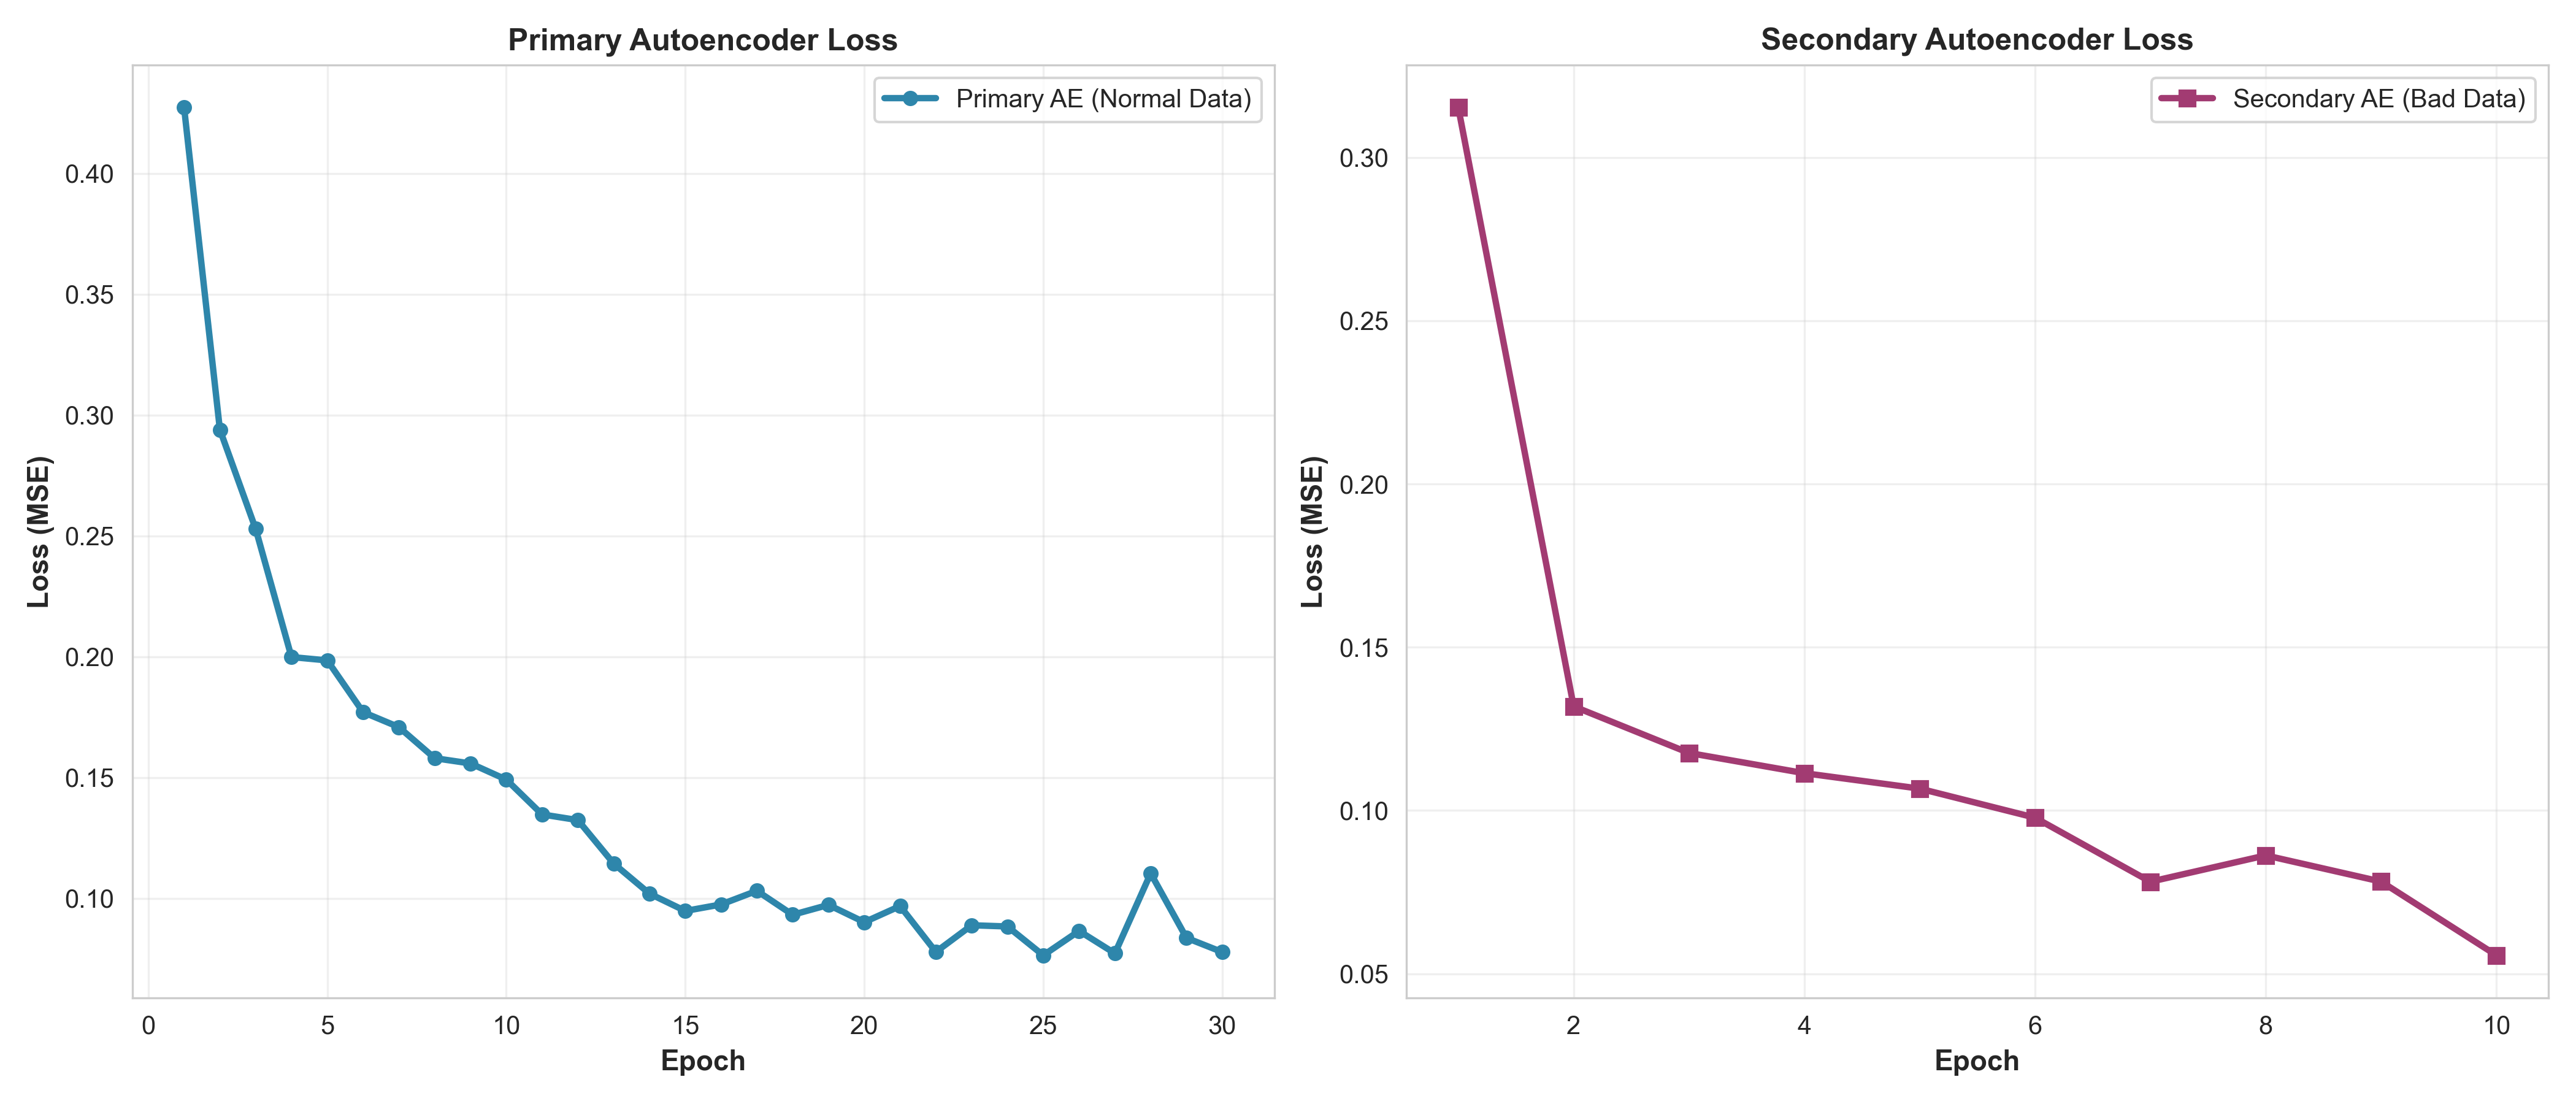
\includegraphics[width=0.8\textwidth]{../evaluation_results/autoencoder_loss_comparison.png}
    \caption{Training Loss (MSE) over Epochs for Primary and Secondary Autoencoders.}
    \label{fig:ae_loss}
\end{figure}

\paragraph{Dual Autoencoder Combination (logical OR).}
Rather than a traditional ensemble where multiple homogeneous models are trained 
on the same data distribution and their outputs are aggregated, this approach 
combines two autoencoders that are \textbf{asymmetrically trained}: the primary AE 
is trained exclusively on benign traffic, while the secondary AE is trained exclusively 
on anomalous traffic. Both models independently receive the same raw test input, and a 
flow is flagged if \textit{either} model classifies it as anomalous (logical \texttt{OR}).

This design exploits complementary detection axes: the primary AE identifies deviations 
from normal behaviour, while the secondary AE identifies similarity to known attack 
patterns. The combination maximises Recall (96.3\%), at the explicit cost of Precision 
(56.8\%).

A known limitation is \textbf{error accumulation}: since the final decision depends on 
the union of two independent classifiers, any misclassification from either model 
propagates directly into the output. A false positive from \textit{either} AE produces 
a false positive in the combined system, which explains the elevated false alarm rate. 
This trade-off is accepted in a security context where missing an attack is far more 
costly than triggering a false alert, but it must be acknowledged and mitigated in 
operational deployments through a human review layer.


\subsection{Selected Model and Rationale}

The \textbf{Dual Autoencoder Combination} was selected as the primary model. Its near-perfect discrimination (AUC-ROC: 0.983) and its ability to detect 96.3\% of attacks position it as the strongest choice for an intrusion detection system. The precision trade-off (57\%) implies a higher false positive rate, which in practice requires a human review layer, an acceptable and recommended operational cost. For contexts where operational efficiency takes priority, the \textbf{Second Autoencoder} remains a strong alternative with a much lower false alarm rate (24\%) at the cost of missing approximately 23\% of attacks.


\section{Preliminary Ethical Considerations}

The development of anomaly detection systems for network traffic raises several ethical concerns that must be addressed from the earliest stages of the project.

\subsection{Privacy and Data Anonymisation}
The CIC-IDS2017 dataset was collected in a controlled environment by the Canadian Institute for Cybersecurity and consists of synthetic network flows generated by simulated user profiles. It therefore contains no real personal data. However, in real-world deployments, the capture of network metadata (IP addresses, ports, traffic volumes) can be sufficient to identify individuals. Any system derived from this work should comply with applicable data protection regulations, such as the \textbf{General Data Protection Regulation (GDPR)}.

\subsection{Algorithmic Bias and Fairness}
Models trained on this dataset reflect the patterns present in synthetic traffic, which may not generalize adequately to diverse, real-world environments. Deployed in production, such models could produce false positives that disproportionately flag legitimate traffic from certain user profiles or network configurations, raising fairness concerns.

\subsection{Consequences of False Negatives}
In the context of network intrusion detection, a \textbf{False Negative} occurs when a malicious flow is incorrectly classified as benign, thereby evading detection. This represents the most critical failure mode of the system: unlike false positives, which cause operational inconvenience, undetected attacks can lead to \textbf{data breaches, infrastructure compromise, or prolonged lateral movement} within a network. The ethical responsibility of deploying such a system therefore requires not only optimizing aggregate metrics such as F1-Score, but explicitly monitoring and bounding the \textbf{False Negative Rate}. Any real-world deployment must define an acceptable risk threshold and incorporate complementary safeguards, such as human-in-the-loop review and layered defenses, to mitigate the consequences of missed detections.


\subsection{Responsible Use}
The anomaly detection techniques developed in this project are intended for \textbf{network protection and cybersecurity}. Nevertheless, the same analytical capabilities could potentially be misused for unauthorised surveillance. Any practical deployment must therefore be accompanied by clear governance policies, audit mechanisms, and human oversight of blocking or alerting decisions.

\section{Adjustments Made Since Deliverable 1}

Based on preliminary findings and empirical obstacles encountered during the practical experimentation phase, several critical refinements to the original project proposal (Deliverable 1) were necessary.

\subsection{Data Management and Memory Constraints}
In Deliverable 1, the dataset was treated conceptually as a static collection. However, during implementation, loading the entire CIC-IDS2017 dataset (over 2.8 million instances) triggered Out-Of-Memory (OOM) failures on local machines, particularly when running algorithms with high computational complexity ($\mathcal{O}(n^2)$) such as the One-Class SVM. To resolve this, we adjusted our operational expectations and implemented a \textbf{20\% Stratified Sampling} strategy. This ensured computational feasibility for local training while rigorously maintaining the native behavioral distribution (roughly 80\% benign, 20\% anomalous) required for unbiased testing.

\subsection{Feature Pruning and Focus}
Initial exploratory analysis revealed that several features extracted by CICFlowMeter were static or uninformative. We introduced a dynamic filtration mechanism that eliminated 8 features demonstrating zero variance. Removing these static attributes reduced computational noise without needing blind dimensionality reduction techniques like PCA. Furthermore, due to formatting inconsistencies observed in network identifiers (IP addresses, ports) and sequential timestamps, we restricted the model's feature space entirely to continuous statistical artifacts.

\subsection{Handling Imbalance and Evaluating Performance}
While Deliverable 1 proposed standard metrics like Precision, Recall, and F1-Score, we quickly realized that global aggregates were deeply misleading on imbalanced data. Instead of using Synthetic Minority Over-sampling Technique (SMOTE) to balance the data, which we deliberately rejected to prevent artificially inflating test metrics and to ensure generalization to zero-day attacks, we revised the evaluation methodology. We adopted a \textbf{Multi-Perspective Evaluation Framework}. This involved testing against both original and synthetically balanced subsets, performing per-class performance breakdowns, and introducing \textbf{AUC-ROC} and \textbf{Balanced Accuracy} as our primary threshold-independent indicators.

\subsection{Evolution of the Modelling Strategy}
Our initial proposal leaned heavily on classical unsupervised techniques (distance-based, density-based, or isolation-based). However, empirical results demonstrated that algorithms like Local Outlier Factor (LOF) suffer severely from the curse of dimensionality in our 70-feature space, performing at near-random levels. To overcome this limitation, we expanded our scope into deep learning by developing PyTorch-based \textbf{Autoencoders}. The superior ability of these neural networks to capture complex, non-linear dependencies fundamentally shifted our approach, culminating in the adoption of an asymmetrically trained \textbf{Dual Autoencoder Combination} rather than relying solely on classical baselines.


\end{document}